% !TeX root = ../technical_paper.tex
\section{原理分析与硬件电路图}

\subsection{系统硬件总体架构}

本系统硬件采用主控制、储能管理和无线监控分层协同的架构。整体上，主控制板以 GD32G553 为核心，负责系统调度、采样管理、控制输出和板间通信；BMS 板以 GD32C113 为核心，负责电池状态采集、保护判定、均衡控制和 SOC 管理；无线监控板以 GD32VW553 为核心，负责运行数据上报、参数交互和远程监测。各功能模块相互独立，并通过标准通信接口连接，使系统在保证功能完整性的同时具备较好的可扩展性和可维护性。

系统硬件设计遵循功能解耦、分层控制和接口统一的原则。主控制层面向整机运行状态，重点完成关键参数采集、控制量计算、功率接口驱动和故障响应；储能管理层面向电池组安全，重点完成单体电压、总电压、电流和温度监测，并结合保护逻辑与均衡控制实现电池状态管理；通信层面则面向远程监控与数据交互，负责运行信息展示、参数配置和日志记录。这样的硬件划分使得高频控制、慢速监测和人机交互彼此独立，避免单一控制器同时承担过多任务造成系统耦合度过高。

从实现角度看，主控制板与 BMS 板之间通过通信总线完成数据交互，主控制板与无线模块之间通过串口完成命令转发和状态上报。主控制板采集到的模拟量主要用于运行状态判断和控制闭环，而 BMS 板采集到的数据主要用于电池保护、均衡决策和电池健康状态评估。无线模块只承担信息交互任务，不直接参与快速功率控制，从而避免无线链路的不确定延迟影响核心控制环路的稳定性。

\subsection{主控制板总体设计}

主控制板的核心器件为 GD32G553RET7。该芯片具备较丰富的 ADC、定时器、通信接口和 GPIO 资源，能够满足系统对多路采样、PWM 输出、通信交互和故障检测的需求。主控制板最小系统包括 8MHz 外部晶振、32.768kHz 低速晶振、复位电路、BOOT 启动选择电路、SWD 下载接口以及各电源引脚附近的去耦电容。每组供电引脚附近均布置 100nF 去耦电容，并在电源入口处布置较大容量电容，以降低数字开关噪声和电源波动对 MCU 工作稳定性的影响。

主控制板预留了多路 HRTIMER PWM 输出接口，用于后续功率级驱动信号输出。虽然三端口功率主回路尚未完成，但控制板已经完成 PWM 输出、故障输入和采样接口的硬件预留。其中，\texttt{HRTIMER\_FLT0} 用作硬件故障输入，可与过流保护信号连接。当外部过流比较或保护电路触发时，故障信号能够直接进入定时器保护通道，使 PWM 输出快速关闭，从而提高系统硬件保护的实时性。

\subsection{主控制板详细电路设计}

\subsubsection{主控最小系统}

主控制板核心器件选用 GD32G553RET7。该芯片具有较丰富的 ADC、HRTIMER、通信接口和 GPIO 资源，能够满足系统对多路采样、PWM 输出、故障检测和数据通信的需求。主控最小系统包括 8MHz 外部高速晶振、32.768kHz 低速晶振、复位电路、BOOT 启动选择电路、SWD 下载调试接口以及电源去耦电容。

在电源完整性设计方面，主控板在每组供电引脚附近均布置 100nF 去耦电容，并在电源入口和关键电源节点布置较大容量电容，用于抑制电源纹波和数字开关噪声。复位电路和 BOOT 电路用于保证系统能够稳定启动，并支持正常运行模式和下载调试模式切换。SWD 接口用于程序下载和在线调试，便于后续对采样、通信和控制逻辑进行联调。

\subsubsection{采样电路设计}

主控制板设计了多路 ADC 采样接口，采样对象包括光伏输入电压 \texttt{V\_PV}、电池电压 \texttt{V\_BAT}、输出电压 \texttt{V\_OUT}、光伏输入电流 \texttt{I\_PV}、电池电流 \texttt{I\_BAT}、输出电流 \texttt{I\_OUT}、MOSFET 温度 \texttt{TEMP\_MOS} 和磁性器件温度 \texttt{TEMP\_MAG}。这些信号经过前端分压、调理或传感器转换后进入 MCU ADC 引脚，用于系统状态判断、闭环控制和保护判定。

从原理图可以看出，各 ADC 输入端均配置了串联电阻和对地电容构成的 RC 滤波网络，其中串联电阻典型值为 $1\,\mathrm{k}\Omega$，滤波电容典型值为 $4.7\,\mathrm{nF}$。该滤波网络的截止频率可近似表示为

\[
f_c=\frac{1}{2\pi RC}.
\]

代入 $R=1\,\mathrm{k}\Omega$、$C=4.7\,\mathrm{nF}$，可得

\[
f_c\approx \frac{1}{2\pi\times1000\times4.7\times10^{-9}}
\approx 33.9\,\mathrm{kHz}.
\]

该截止频率能够抑制采样线上的高频噪声和开关毛刺，同时不会明显影响电压、电流和温度等慢变量的采样响应。电压类信号通过分压网络映射至 ADC 允许范围，电流类信号通过采样电阻或电流传感器转换为电压信号，温度类信号则通过热敏电阻或温度采样网络获得。主控制器在软件中根据比例系数完成物理量还原，从而得到实际电压、电流和温度值。

\subsubsection{PWM 与硬件保护接口}

主控制板预留了多路 HRTIMER PWM 输出接口，包括 \texttt{PWM\_M1}、\texttt{PWM\_M2}、\texttt{PWM\_M3}、\texttt{PWM\_MA} 以及若干备用 PWM 通道。这些接口用于后续主功率级驱动信号输出。虽然三端口功率变换主回路尚未完成，但主控制板已经完成了控制信号输出和故障保护输入的硬件预留。

硬件保护接口中，\texttt{HRTIMER\_FLT0} 用于接收外部过流或故障关断信号。当外部比较器、驱动器或保护电路检测到异常时，故障信号可直接送入 HRTIMER 故障输入通道，使 PWM 输出快速关闭。与单纯依赖软件中断处理相比，硬件保护链路具有响应速度快、确定性高的优点，适合用于过流、短路等需要快速关断的故障场景。

\subsubsection{通信接口设计}

主控制板同时设计了 CAN、UART 和 I2C 等通信接口。CAN 接口用于主控制板与 BMS 板之间的数据交互，收发器采用 TCAN1057AVDRQ1。原理图中 CANH 和 CANL 线上布置了保护器件和终端匹配网络，两只 $60.4\,\Omega$ 电阻构成等效 $120\,\Omega$ 终端电阻，有利于减小差分通信过程中的信号反射和波形畸变。

UART 接口主要用于主控制板与 GD32VW553 无线模块之间的数据交互。主控制板将系统运行数据、BMS 状态和故障信息整理后，通过串口发送至无线模块，再由无线模块上传至上位机或监控界面。I2C 接口作为板级扩展接口，可用于后续连接传感器、存储器或其他低速外设。通过多种通信接口的组合，主控制板能够同时完成实时控制、状态采集和远程监控数据转发。

\subsection{BMS 硬件设计}

% TODO: 插入BMS系统框图
\begin{figure}[htbp]
  \centering
  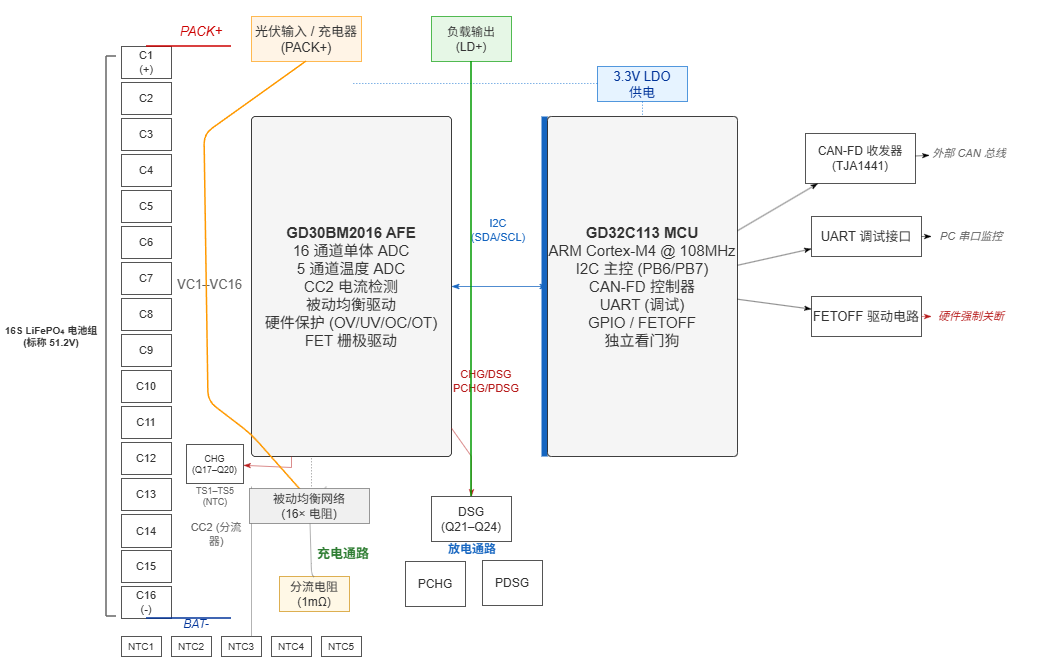
\includegraphics[width=0.95\textwidth]{images/流程图架构图/BMS硬件架构.drawio.png}
  \caption{BMS系统框图}
  \label{fig:bms_system_diagram}
  \vspace{0.2em}
  {\small 资料来源：作者绘制。}
\end{figure}

\subsubsection{BMS 主控最小系统}

BMS 板主控芯片选用 GD32C113CBT6，负责 BMS 状态机运行、保护逻辑判断、均衡策略执行、CAN 通信以及与 AFE 芯片的数据交互。BMS 主控最小系统包括 8MHz 外部晶振、复位电路、BOOT 电路、SWD 下载接口、电源去耦电容和状态指示灯。

GD32C113 与 GD30BM2016 之间通过 I2C 总线进行通信，主控周期性读取电池电压、电流、温度和状态信息，并根据保护阈值和均衡策略进行判断。BMS 板还设计了 ALERT、FETOFF 等关键信号接口，用于接收 AFE 异常提示或执行硬件关断。通过 MCU 与 AFE 的分工，BMS 能够在保证采样精度的同时实现较完整的保护和管理功能。

\subsubsection{AFE 采样电路}

BMS 板采用 GD30BM2016 作为电池监测 AFE 芯片，负责 16S 电池组的单体电压采集、电流检测、温度采集和保护相关信号输出。原理图中电池采样线从 \texttt{CELL0} 至 \texttt{CELL16} 接入，对应 AFE 的 \texttt{VC0} 至 \texttt{VC16} 引脚。每一路采样线上均配置滤波电容和保护器件，用于降低采样线噪声并抑制异常尖峰。

温度采样部分通过多个热敏电阻接口实现，包括电池包中心温度、MOSFET 温度和分流电阻温度等测量点。温度数据用于过温保护、运行状态判断和故障记录。AFE 将采集到的电压、电流、温度和状态信息传递给 BMS 主控，主控再根据运行状态决定是否允许充电、放电或均衡。

\begin{figure}[htbp]
  \centering
  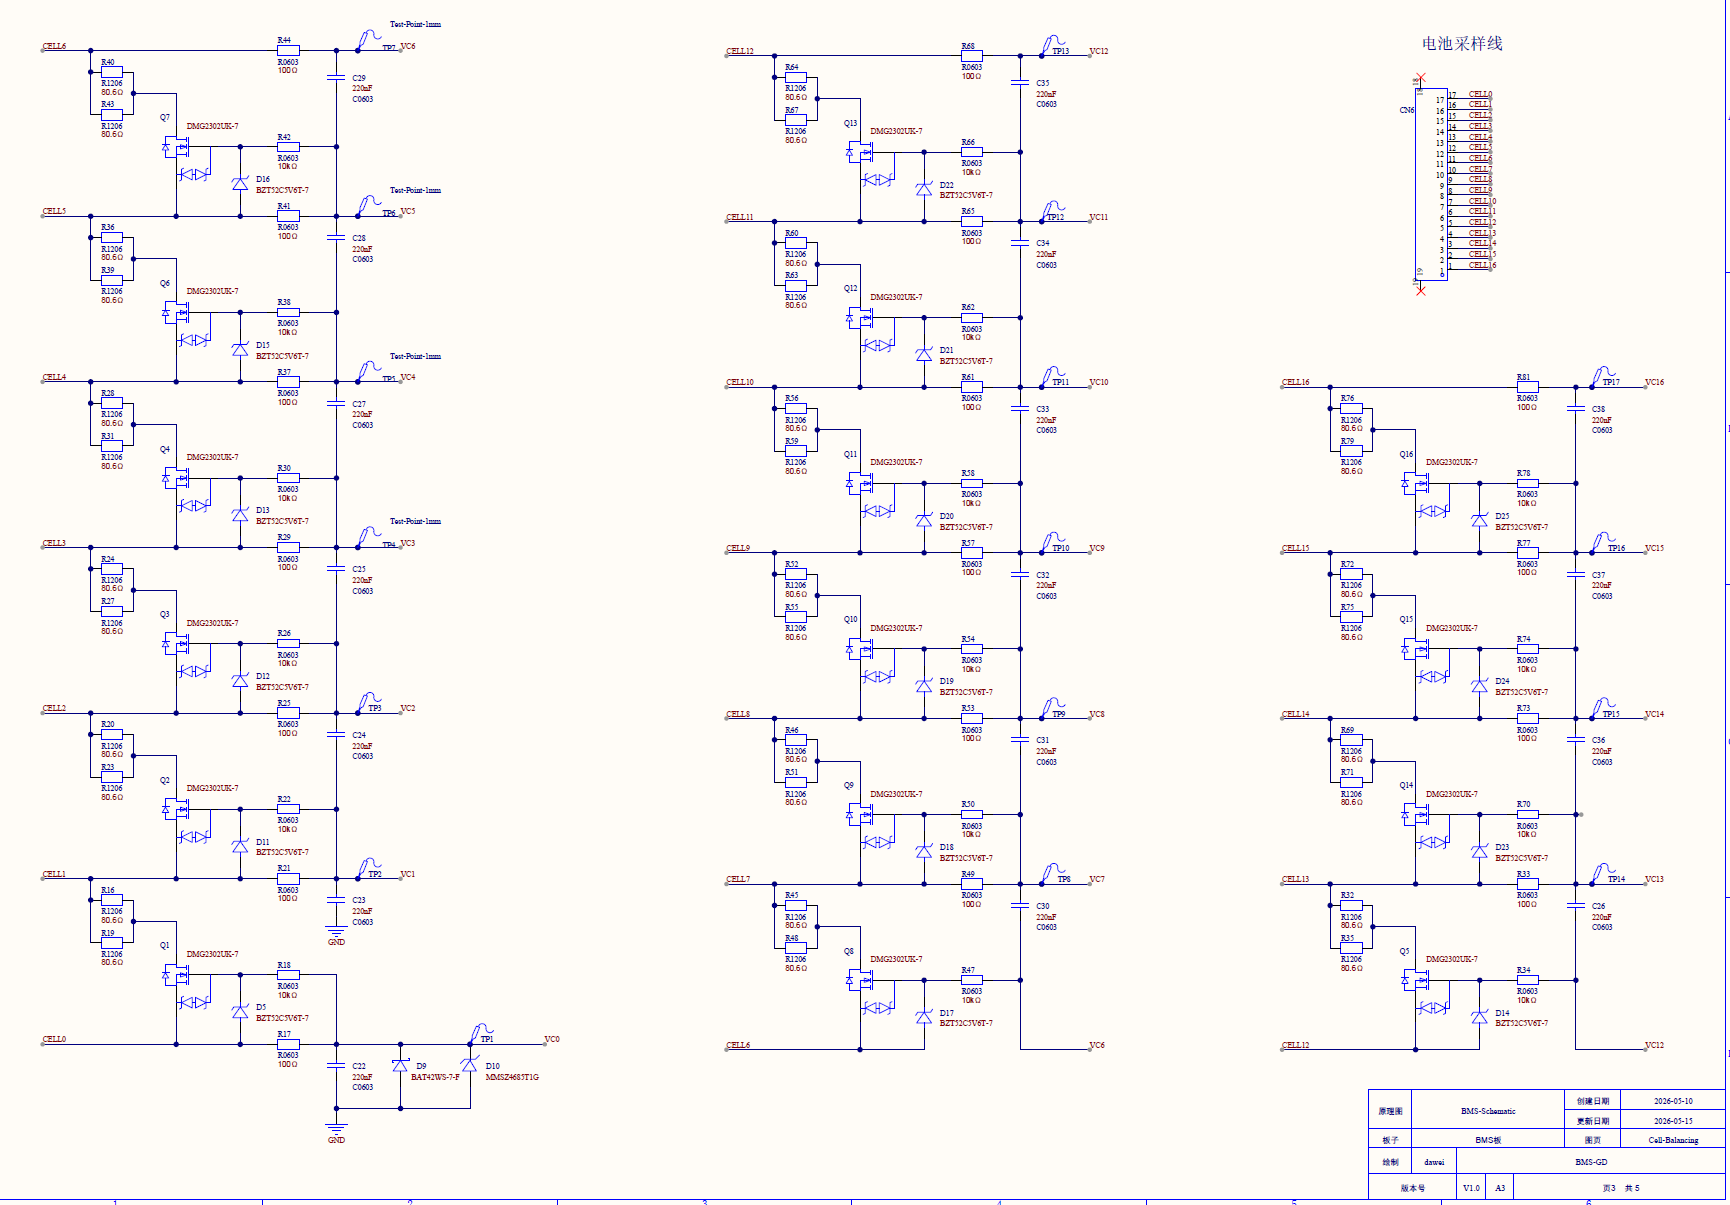
\includegraphics[width=0.95\textwidth]{images/BMS板原理图/bms采样电路.png}
  \caption{AFE采样电路}
  \label{fig:afe_circuit}
  \vspace{0.2em}
  {\small 资料来源：作者绘制。}
\end{figure}

\subsubsection{电流检测电路}

BMS 电流检测采用低阻值分流电阻方式。原理图中使用两只 $2\,\mathrm{m}\Omega$ 采样电阻并联，等效采样电阻为

\[
R_{shunt}=\frac{2\,\mathrm{m}\Omega}{2}=1\,\mathrm{m}\Omega.
\]

当电池电流流过分流电阻时，产生的采样电压为

\[
U_{shunt}=I\times R_{shunt},
\]

对应功率损耗为

\[
P_{shunt}=I^2\times R_{shunt}.
\]

AFE 内部集成可编程增益放大器对分流电阻电压进行放大。以 GD30BM2016 为例，其电流检测通道增益典型值为 $20\,\mathrm{V/V}$，对应 $1\,\mathrm{m}\Omega$ 分流电阻的满量程电流可估算为

\[
I_{\max}=\frac{V_{\mathrm{ADC\_max}}}{G\times R_{shunt}}
=\frac{3.3}{20\times0.001}
=165\,\mathrm{A},
\]

其中 $V_{\mathrm{ADC\_max}}$ 为 AFE 内部 ADC 满量程电压，$G$ 为增益。该量程满足样机阶段充放电电流监测需求。电流分辨率为

\[
\Delta I=\frac{V_{\mathrm{LSB}}}{G\times R_{shunt}},
\]

其中 $V_{\mathrm{LSB}}$ 为 ADC 最低有效位电压。增益越高分辨率越好，但量程相应减小，需在实际应用中权衡选择。

采用两只采样电阻并联可以降低等效阻值，减小大电流工况下的压降和功率损耗，同时分担单个器件的热应力。该电流检测方式结构简单、可靠性高，适合用于 BMS 充放电电流监测和保护判断。

\subsubsection{均衡电路设计}

BMS 板采用被动均衡方案，每节电池对应一路均衡支路。均衡支路由 DMG2302UK-7 MOSFET、放电电阻、栅极电阻和下拉电阻构成。当某一节电池电压高于均衡阈值时，BMS 控制对应 MOSFET 导通，使该单体通过电阻释放部分能量，从而逐步减小单体间电压差。

原理图中均衡电阻采用 $80.6\,\Omega$。当单体电压接近满充电压 $3.65\,\mathrm{V}$ 时，均衡电流可估算为

\[
I_{bal}=\frac{U_{cell}}{R_{bal}}
=\frac{3.65}{80.6}
\approx45\,\mathrm{mA}.
\]

对应均衡电阻功耗为

\[
P_{bal}=\frac{U_{cell}^2}{R_{bal}}
=\frac{3.65^2}{80.6}
\approx0.165\,\mathrm{W}.
\]

因此，采用 1206 封装均衡电阻能够提供较合理的功率余量。该均衡电流不追求快速大电流均衡，而是以安全、稳定和低成本为目标，适合样机阶段对电池一致性进行维护。

\subsubsection{充放电 MOSFET 驱动与保护电路}

BMS 充放电功率通路采用 CRSS028N10N 作为主功率 MOSFET。该器件承担电池包充放电通路的导通与关断任务，其选型主要考虑耐压、导通电阻、连续电流能力和散热能力。16S 磷酸铁锂电池组标称电压为

\[
U_{nom}=16\times3.2\,\mathrm{V}=51.2\,\mathrm{V},
\]

满充电压为

\[
U_{max}=16\times3.65\,\mathrm{V}=58.4\,\mathrm{V}.
\]

因此，功率 MOSFET 的耐压需要高于电池包最高电压，并留有开关尖峰和异常工况余量。CRSS028N10N 属于 100V 等级 MOSFET，$V_{DS}=100\,\mathrm{V}$，电压裕量为

\[
K_V=\frac{V_{DS}}{U_{max}}=\frac{100}{58.4}\approx1.71,
\]

满足工程设计中对电压裕量不低于 1.5 倍的要求。其导通电阻 $R_{DS(on)}=2.8\,\mathrm{m}\Omega$（典型值，$V_{GS}=10\,\mathrm{V}$），额定连续漏极电流 $I_D=200\,\mathrm{A}$（$T_C=25\,\mathrm{°C}$）。以额定充放电电流 $20\,\mathrm{A}$ 估算，单管导通损耗为

\[
P_{cond}=I^2\times R_{DS(on)}=20^2\times2.8\times10^{-3}=1.12\,\mathrm{W}.
\]

通过多颗 MOSFET 并联或分组布置，可以降低等效导通电阻并分担热损耗。以两管并联为例，等效导通电阻降至 $1.4\,\mathrm{m}\Omega$，对应导通损耗约 $0.56\,\mathrm{W}$，结合封装热阻和散热条件，结温可控制在安全范围内。原理图中还设置了预充电支路，利用预充 MOSFET 和限流电阻在主通路闭合前对母线电容进行缓慢充电，降低上电瞬间的浪涌电流，保护电池、MOSFET 和后级电路。

驱动与关断逻辑部分采用小信号 MOSFET、限流电阻、下拉电阻和二极管组成。BSS84AK、BSS123NH6327 等器件用于完成逻辑电平转换、栅极拉低和保护信号传递。当 AFE 或 MCU 判断出现过压、过流、过温、通信异常或其他故障时，可通过驱动网络关闭充放电 MOSFET，使电池包进入安全状态。

\begin{figure}[htbp]
  \centering
  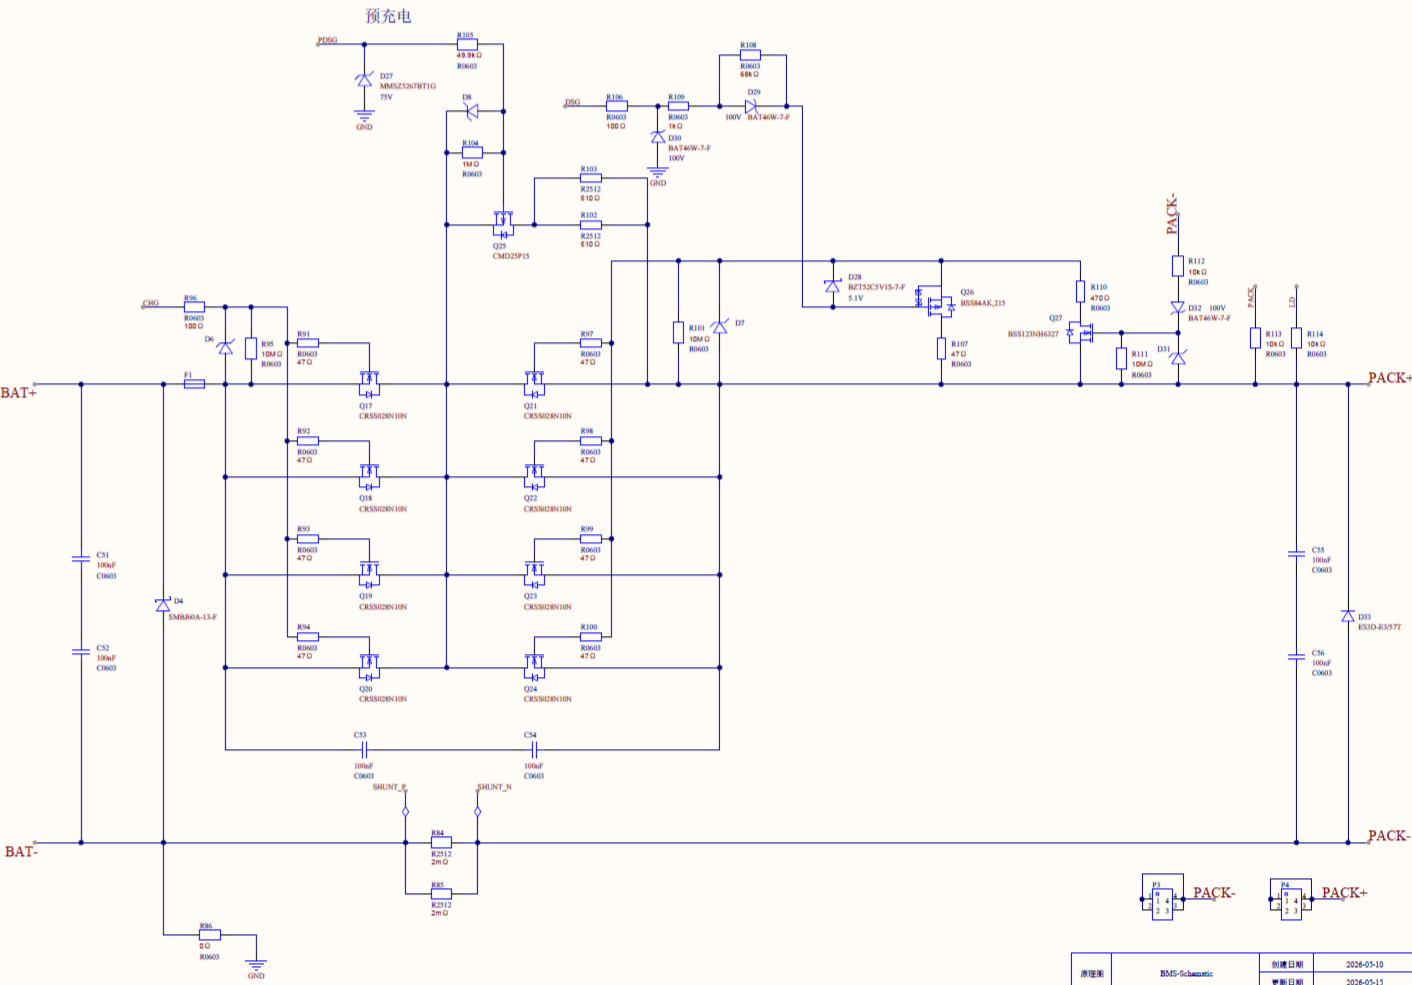
\includegraphics[width=0.95\textwidth]{images/BMS板原理图/bms充放电和保护电路.png}
  \caption{充放电MOSFET驱动与保护电路}
  \label{fig:mos_circuit}
  \vspace{0.2em}
  {\small 资料来源：作者绘制。}
\end{figure}

\subsection{辅助电源设计}

主控制板辅助电源由电池包输入经两级降压和一级 LDO 构成。第一级采用 LMR38020 将电池包电压降至 $12\,\mathrm{V}$；第二级采用 TPS54202 将 $12\,\mathrm{V}$ 降至 $5\,\mathrm{V}$；最后通过 LDO（SCJA1117B-3.3）生成 $3.3\,\mathrm{V}$ 逻辑电源。对于 16S LFP 电池包，输入电压约为 $40\,\mathrm{V}$ 至 $58.4\,\mathrm{V}$，因此 12V 降压级占空比范围约为

\[
D_{12V}=\frac{12}{58.4}\sim\frac{12}{40}
\approx20.5\%\sim30.0\%.
\]

5V 降压级的占空比约为

\[
D_{5V}=\frac{5}{12}\approx41.7\%.
\]

该两级降压结构能够减小单级降压的压差压力，提高系统供电稳定性。3.3V 由 LDO 产生，主要用于降低开关电源纹波对 MCU、ADC 和通信接口的影响。若 3.3V 负载电流为 $I_{3.3}$，则 LDO 功耗为

\[
P_{LDO}=(5-3.3)\times I_{3.3}.
\]

BMS 板辅助电源采用 LMR38010SDDAR 将电池包电压降至 $5\,\mathrm{V}$，再通过 SCJA1117B-3.3-A 生成 $3.3\,\mathrm{V}$。BMS 板长期接入电池包，因此电源部分不仅要求宽输入范围和较高效率，还需要具备良好的可靠性。原理图中在输入端布置了保险丝和 TVS 管，其中 SMBJ60A-13-F 用于抑制电池端瞬态过压。由于 16S LFP 电池包满充电压为 $58.4\,\mathrm{V}$，选用 60V 等级 TVS 能够在正常工作时避免误动作，在异常浪涌时提供钳位保护。

\subsection{功率器件选型与计算}

系统功率器件选型遵循耐压留有余量、导通损耗较低、热设计可控和保护优先的原则。对于直接连接电池包的器件，其耐压等级必须高于 $58.4\,\mathrm{V}$ 的满充电压，并考虑开关尖峰、线束寄生参数和异常工况下的电压冲击。对于长期承载电流的 MOSFET、采样电阻和均衡电阻，需要通过功耗公式估算其热应力，并结合封装功率能力进行校核。

主功率 MOSFET 的关键指标为耐压 $V_{DS}$、导通电阻 $R_{DS(on)}$、连续漏极电流和封装热阻。由于导通损耗随电流平方增加，因此在较大电流场景下，降低 $R_{DS(on)}$ 和合理并联 MOSFET 是减小温升的重要方法。分流采样电阻的关键指标为阻值精度、温漂和额定功率；均衡电阻的关键指标为阻值、封装功率和温升；TVS 器件的关键指标为反向工作电压、钳位电压和浪涌功率能力。

功率板隔离驱动采用 UCC21540ADWKR 双通道隔离栅极驱动芯片。该器件的关键参数包括：隔离耐压 $5.7\,\mathrm{kV_{RMS}}$（增强型隔离），峰值驱动电流 $4\,\mathrm{A}$ / $6\,\mathrm{A}$（拉/灌），传播延迟典型值 $19\,\mathrm{ns}$，CMTI（共模瞬态抗扰度）$\ge150\,\mathrm{V/ns}$。选型依据如下：

\begin{itemize}[leftmargin=*,itemsep=0.3ex]
  \item \textbf{隔离耐压}：功率板存在高 $dv/dt$ 开关节点，驱动侧与功率侧需要足够的电气隔离。UCC21540 的 $5.7\,\mathrm{kV_{RMS}}$ 隔离耐压满足低压功率变换场景的安全要求。
  \item \textbf{驱动能力}：IRFP4668PBF 等功率 MOSFET 的栅极电荷 $Q_g\approx200\,\mathrm{nC}$，以 $4\,\mathrm{A}$ 峰值电流驱动时，上升时间约 $Q_g/I_{peak}=50\,\mathrm{ns}$，满足开关频率下的驱动速度要求。
  \item \textbf{CMTI}：三端口变换器开关节点的 $dv/dt$ 可达数 $kV/\mu s$，UCC21540 的高 CMTI 保证了在快速开关过程中隔离信号不被共模噪声干扰。
\end{itemize}

以 BMS 功率通路为例，电池组最高电压为 $58.4\,\mathrm{V}$，选用 100V 等级 MOSFET 的电压裕量 $K_V\approx1.71$，满足工程设计要求。均衡支路功耗约 $0.165\,\mathrm{W}$，1206 封装电阻满足样机阶段需求。分流电阻并联后等效阻值 $1\,\mathrm{m}\Omega$，在保证采样分辨率的同时降低了功率损耗。

综合来看，当前硬件设计已经围绕 16S 磷酸铁锂电池系统完成了控制、采样、保护、通信、驱动和辅助电源的基础平台搭建。虽然三端口功率变换主回路尚未完成实物闭环实现，但控制板与 BMS 板已经为后续充放电实验、功率级接入和整机联调提供了完整的硬件支撑。

\subsection{本章小结}

本章对系统硬件设计进行了说明。主控制板完成了 GD32G553 最小系统、ADC 采样接口、PWM 输出接口、硬件故障保护输入、CAN 通信和 UART 通信等硬件设计；BMS 板完成了 GD32C113 主控、GD30BM2016 AFE 采样、电流检测、温度采集、单体均衡、充放电 MOSFET 驱动和保护关断电路设计；辅助电源部分完成了电池包到 12V、5V 和 3.3V 的多级供电设计。通过功率器件选型与计算可知，系统关键器件在耐压、功耗和保护能力方面能够满足 16S LFP 电池系统的基础需求，为后续主功率部分实现和整机实验验证奠定了硬件基础。
